\section{Qu'est ce que l'apprentissage automatique ?}

L' \textbf{apprentissage automatique}, ou \textit{Machine Learning} en anglais, est la discipline scientifique dont l'objectif est d'analyser une certaine quantité de données (de préférence assez grande) afin d'en déduire un modèle \textit{statistique} permettant d'\textbf{inférer} un résultat de \textbf{classification}.

On distingue principalement deux grands types d'apprentissage :
\begin{itemize}
	\item \textbf{Apprentissage Supervisé}
	\item \textbf{Apprentissage Non-Supervisé}
\end{itemize}
\vspace{3mm}

Il existe d'autres modes d'apprentissage, moins courant, sur lesquels je ne m'étendrai pas :
\begin{itemize}
	\item \textbf{Apprentissage Semi-Supervisé}
	\item \textbf{Apprentissage Par Renforcement}
	\item \ldots
\end{itemize}
\vspace{3mm}
 
Ses applications sont très larges et vont de l'\textit{analyse prévisionnelle financière}, à la \textit{détection de comportements anormaux} (Sécurité Informatique, Fraude Financière, \ldots), en passant par l'étude de la \textit{génétique} ou encore les \textit{moteurs de recommandation} comme ceux d'Amazon ou Netflix. 

 \begin{figure}[H]
    \centering
    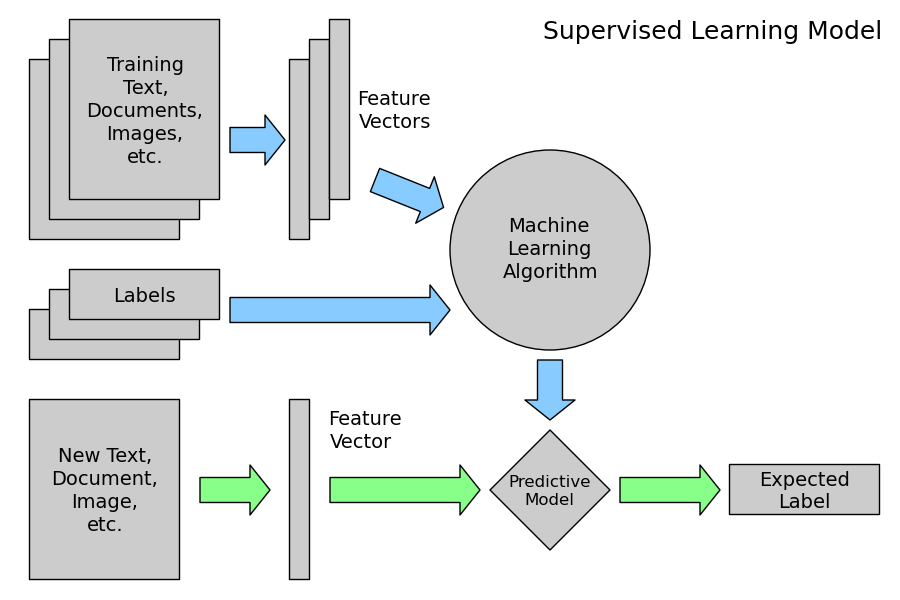
\includegraphics[height=5.5cm]{supervisedLearning.png}
	\caption{Schéma de fonctionnement d'un apprentissage supervisé~-~Source: \href{http://www.astroml.org/sklearn_tutorial/general_concepts.html\#supervised-learning-model-fit-x-y}{AstroML}}\label{image.supervisedLearning} 
\end{figure}

 \begin{figure}[H]
    \centering
    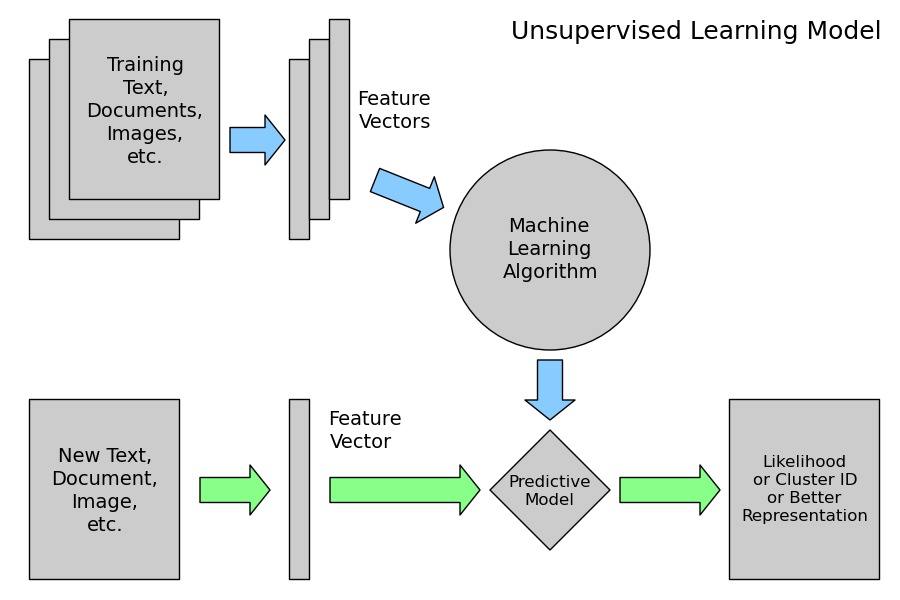
\includegraphics[height=5.5cm]{unsupervisedLearning.png}
	\caption{Schéma de fonctionnement d'un apprentissage non supervisé~-~Source: \href{http://www.astroml.org/sklearn_tutorial/general_concepts.html\#unsupervised-learning-model-fit-x}{AstroML}}\label{image.unsupervisedLearning} 
\end{figure}


\section{L'apprentissage Supervisé}

L'\textit{apprentissage supervisé} est l'une des méthodes des plus couramment utilisés dans le cadre de l'apprentissage automatique.

Pour le mettre au point, le tester et l'utiliser, nous avons besoin de trois jeux de données :

\begin{itemize}
	\item Pour la phase dite d'\textbf{apprentissage}, chaque exemple est constitué d'une paire : Un \textbf{vecteur de variables} et la \textbf{valeur de sortie} désirée.\\
	
	\item Pour la phase dite de \textbf{test}, chaque exemple est également constitué d'une paire : Un \textbf{vecteur de variables} et la \textbf{valeur de sortie} que l'algorithme devrait donner en théorie.\\ 
	En comparant la sortie théorique et celle fourni par l'algorithme sur l'ensemble du jeu de test, on obtient un indicateur de précision sur notre méthode d'apprentissage.\\
	
	\item Pour la dernière phase, dite de \textbf{production ou d'exploitation}, seul le \textbf{vecteur de variables} est connu. Nous utilisons à présent l'algorithme d'apprentissage automatique pour \textbf{inférer} le résultat de \textbf{classification}.

\end{itemize}
\vspace{3mm}

Il est important de comprendre que l'apprentissage supervisé requiert l'intervention d'un \textbf{expert} du domaine afin d'obtenir la \textit{vraie classe} de chacun des exemples des jeux de test et d'apprentissage. Cette connaissance est nécessaire à la construction des jeux de données.

\vspace{3mm}

Il existe de nombreux algorithmes permettant de mettre en place un apprentissage supervisé. On retrouve, pour les plus connus, les algorithmes suivants : 

\begin{itemize}
	\item SVM : Séparateurs à Vaste Marge (en anglais: \textit{Support Vector Machine})\\
	
	\item KNN : Méthode des k plus proches voisins (en anglais:  K-Nearest Neighbor).\\
	
	\item Arbres de Décision.\\
	
	\item Réseaux Neuronaux (Perceptron Multicouches).\\
	
	\item Régression Linéaire.\\
	
	\item Régression Logistique.\\
	
	\item Classification naïve bayésienne.\\
	
	\item Analyse discriminante linéaire.\\
	
	\item  \ldots
	
\end{itemize}
\clearpage	
	
\section{L'apprentissage Non Supervisé}

L'\textit{apprentissage non supervisé} est un autre des modes d'apprentissage des plus couramment utilisés dans le cadre de l'apprentissage automatique.

A l'inverse de l'apprentissage supervisé, la \textit{connaissance expert} n'est pas requise. Il n'y a pas de \textit{sortie a priori}. L'objectif n'est donc pas d'inférer un résultat sur un ensemble d'étiquettes connues, mais bien de diviser un \textbf{groupe hétérogène de données}, en sous-groupes (ou \textit{clusters}) de manière à regrouper les données qui semblent les plus similaires entre elles. À l'inverse des données peu similaires devraient être dans des groupes distincts. L'\textbf{objectif} d'un algorithme d'\textit{apprentissage automatique non supervisé} est d'\textbf{extraire de manière organiser} un \textit{ensemble de connaissances} sur les données traitées.


Pour le mettre au point, le tester et l'utiliser, nous avons toujours besoin de trois jeux de données, mais qui sont cette fois ci identiques dans leur construction :

\begin{itemize}
	\item Pour la phase dite d'\textbf{apprentissage}, chaque exemple est constitué d'un \textbf{vecteur de variables}.\\
	
	\item Pour la phase dite de \textbf{test}, chaque exemple est également constitué d'un \textbf{vecteur de variables}.\\
	
	\item Pour la dernière phase, dite de \textbf{production ou d'exploitation}, toujours un ensemble d'exemples constitués d'un \textbf{vecteur de variables}.

\end{itemize}
\vspace{3mm}


Il existe de nombreux algorithmes permettant de mettre en place un apprentissage non supervisé. On retrouve, pour les plus connus, les algorithmes suivants : 

\begin{itemize}
	\item Algorithme EM : Espérance-Maximisation (en anglais: \textit{Expectation-Maximisation})/\\
	
	\item ACP : Analyse en Composantes Principales.\\
	
	\item K-moyennes (en anglais: \textit{K-Means}).\\
	
	\item Réseaux Neuronaux.\\
	
	\item  \ldots
	
\end{itemize}